\documentclass[conference,a4paper]{IEEEtran}

\usepackage{graphicx}
\usepackage{amsmath}
\usepackage{booktabs}
\usepackage[caption=false,font=footnotesize]{subfig}
\usepackage{siunitx}
\usepackage{tikz}
\usetikzlibrary{positioning,arrows.meta}
\usepackage[hidelinks]{hyperref}
\usepackage[left=1.15cm,right=1.15cm,top=0.95cm,bottom=1.22cm]{geometry}   % visible margin 1.15 cm on all sides (top/bottom offset for topskip and descenders)
\usepackage{fontspec}
\newfontfamily\titlefont{Helvetica}   % Helvetica for the title only

% bold headings, IEEEtran conference spacing kept
\makeatletter
\def\section{\@startsection{section}{1}{\z@}{1.5ex plus 1.5ex minus 0.5ex}{0.7ex plus 1ex minus 0ex}{\normalfont\normalsize\centering\bfseries}}
\def\subsection{\@startsection{subsection}{2}{\z@}{1.5ex plus 1.5ex minus 0.5ex}{0.7ex plus .5ex minus 0ex}{\normalfont\normalsize\itshape\bfseries}}
\def\paragraph{\@startsection{paragraph}{4}{2\parindent}{0ex plus 0.1ex minus 0.1ex}{0ex}{\normalfont\normalsize\itshape\bfseries}}
\makeatother

% figures are read straight from the repository (compile from latex/Final paper/)
\graphicspath{{../../media/}{../../scripts and outputs/tier_1/output/}{../../scripts and outputs/tier_3/output/}}

\newcommand{\repo}{https://github.com/Shass27/curiosity-perseverance-wheel-fea}
\newcommand{\tree}{\repo/tree/main}
\newcommand{\blob}{\repo/blob/main}

\begin{document}

\title{\titlefont\bfseries{From Curiosity to Perseverance: Failure Analysis and Surrogate Modelling of Mars Rover Wheel Skin Stress}}

\author{\IEEEauthorblockN{Pabitra Kumar Sahoo, Ridam Bagul, Sibasis Panda and Shaswath S}
\IEEEauthorblockA{Department of Mechanical and Aerospace Engineering\\
Indian Institute of Technology Hyderabad, India\\
\href{\repo}{\texttt{github.com/Shass27/curiosity-perseverance-wheel-fea}}~\cite{repo}}}

\maketitle

\begin{abstract}
The thin aluminium skin of the Curiosity rover's wheels has cracked in service, mostly where it meets the grousers. We study why, and how much the Perseverance redesign helps, in two steps. First, a flat skin segment between two grousers is loaded by a rock patch of radius 2--\SI{10}{mm} at \SI{400}{N} and solved with a clamped stepped-beam model and with Ansys FEA on three meshes. On the converged \SI{0.1}{mm} mesh the junction stress is 132--\SI{137}{MPa}, above the \SI{106}{MPa} fatigue limit of Al 7075-T7351 for every rock size. The beam model under-predicts the centre stress ($C_c = 1.07$--$1.47$) and over-predicts the junction stress ($C_j \approx 0.7$), so it is a first guide and not a design check. Second, 440 FEA solutions of the curved R250 wheel panel (five grouser features, two skin thicknesses, three grouser angles, three fillet radii, five patch radii) are used to train a surrogate built from principal component analysis and Gaussian-process regression. On unseen geometries it predicts the peak stress with a median error of 3.1\% and its 95\% band holds the true peak in 94\% of cases.
\end{abstract}

\begin{IEEEkeywords}
Mars rover wheel, finite element analysis, fatigue, mesh convergence, stress concentration, surrogate model, Gaussian process, PCA
\end{IEEEkeywords}

% ---------------------------------------------------------------
\section{Introduction}

NASA/JPL mission reports have documented punctures and cracks in the wheels of the Curiosity rover after driving over sharp, embedded rocks~\cite{nasa}. A rock pressing on the thin aluminium skin between two chevron-shaped grousers bends it like a clamped plate, with the largest stress under the rock and at the skin--grouser fillet. Perseverance was given a thicker skin and a revised grouser pattern, but how much each change helps is not obvious.

This paper asks two questions. For a given rock sharpness, how large are the junction and centre stresses on a Curiosity-like skin, and can a hand calculation predict them? And how far do the Perseverance changes reduce the stress, across a design space that is too large to mesh and solve point by point? We answer the first with an analytical model checked against a mesh-converged FEA, and the second with a 440-case FEA dataset and a real-time surrogate model. Full derivations and discussion are in the detailed reports~\cite{rep1,rep2}.

\begin{figure}[!t]
  \centering
  \subfloat[Region of the wheel analysed]{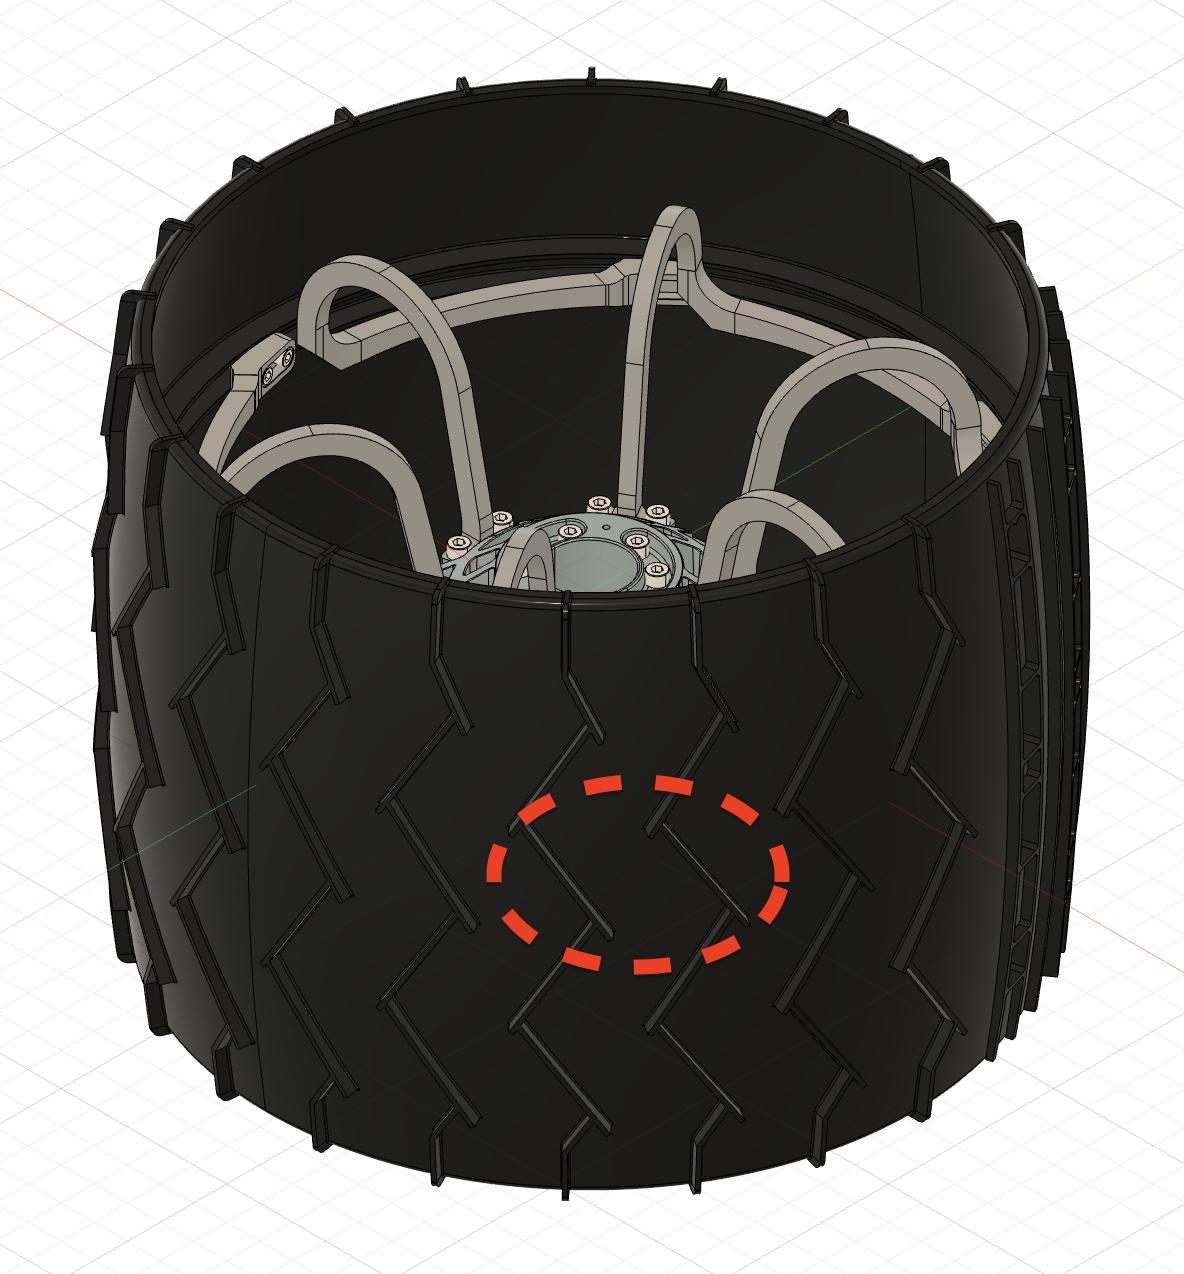
\includegraphics[width=0.40\columnwidth]{analysis_location.png}}\hfill
  \subfloat[Flat skin segment with load patch]{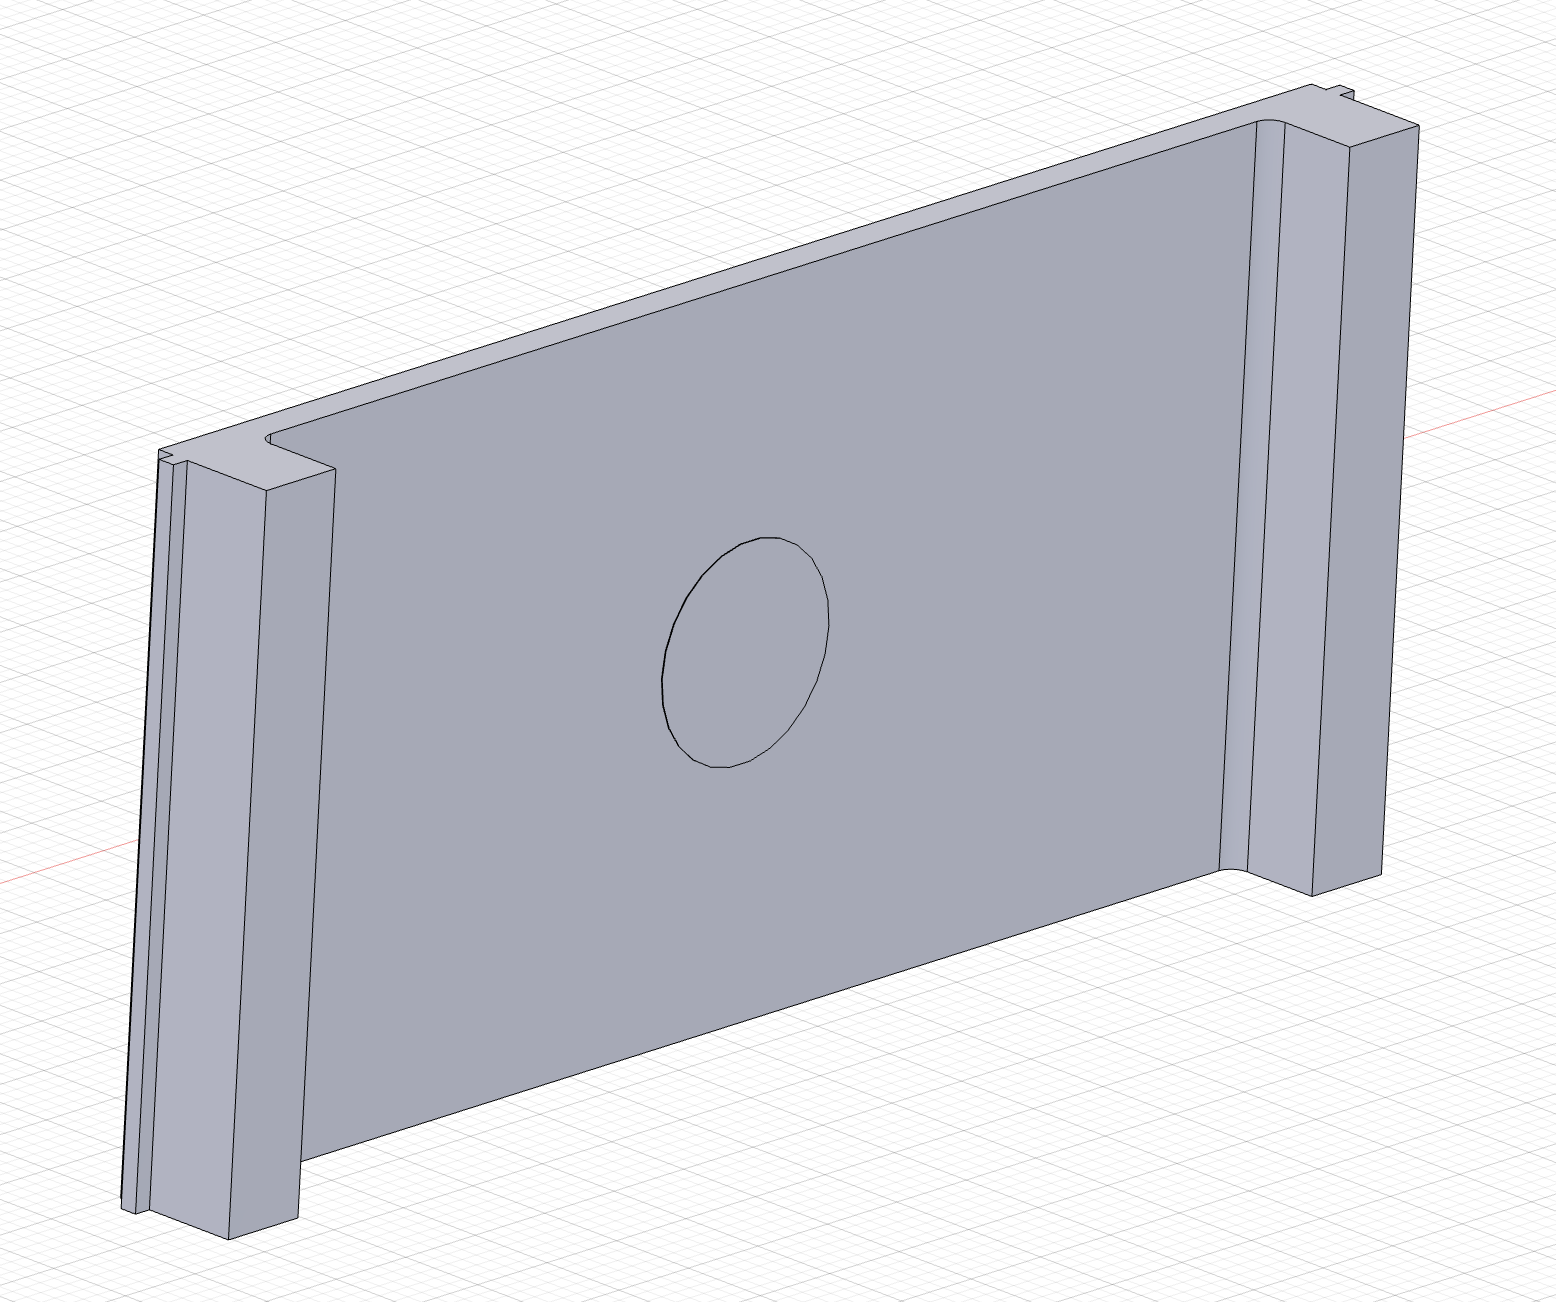
\includegraphics[width=0.56\columnwidth]{analysis_segment.png}}
  \caption{Location of the analysed segment and the CAD model of Section~\ref{sec:flat}.}
  \label{fig:location}
\end{figure}

% ---------------------------------------------------------------
\section{Wheel Segment and Load Model}

\subsection{Flat-skin segment (Curiosity)}\label{sec:flat}
The segment (Fig.~\ref{fig:location}) is a $t = \SI{2}{mm}$ skin between two grouser blocks, each \SI{5}{mm} wide and \SI{7.5}{mm} deep, joined to the skin through an R\SI{1}{mm} fillet. The span is $L = \SI{83}{mm}$, the width is $b = \SI{40}{mm}$ and both end faces are fixed. A uniform pressure acts on a circular patch of radius $a = 2, 4, 6, 8, \SI{10}{mm}$ at mid-span, where a smaller $a$ stands for a sharper rock. The design load is \SI{400}{N}; the FEA was solved at \SI{300}{N} and scaled by $4/3$, which is valid because the model is linear-elastic. The material is Al 7075-T7351 ($E = \SI{72}{GPa}$, $\nu = 0.33$) with a fatigue limit of $\sigma_f = \SI{106}{MPa}$.

\subsection{Curved R250 panel (Curiosity to Perseverance)}
The second study uses the real curved geometry: a \SI{45}{\degree} arc of the R250 wheel panel with its ends fixed and \SI{300}{N} on a patch of radius $R$ at the panel centre. Five grouser features are modelled (Fig.~\ref{fig:features}), each over skin thickness $t \in \{2, 7.5\}$\,mm, grouser angle $s \in \{10, 12, 15\}$\,\si{\degree} (plus \SI{6}{\degree} for one Feature~4 and one Feature~5 geometry), fillet radius $r \in \{1, 3, 5\}$\,mm and $R \in \{2, \dots, 10\}$\,mm. Feature~1 at \SI{2}{mm} is taken as representative of Curiosity and Feature~4 at \SI{7.5}{mm} of Perseverance; neither is claimed to be the exact flight geometry. Of the 458 solved cases, 18 Feature~5 cases with unverified load areas are excluded (\href{\blob/Simulation\%20results/NOTE.md}{\texttt{NOTE.md}}), leaving 440. Sample runs of both models are shown in Fig.~\ref{fig:ansys}.

\begin{figure*}[!t]
  \centering
  \subfloat[F1 (Curiosity-like)]{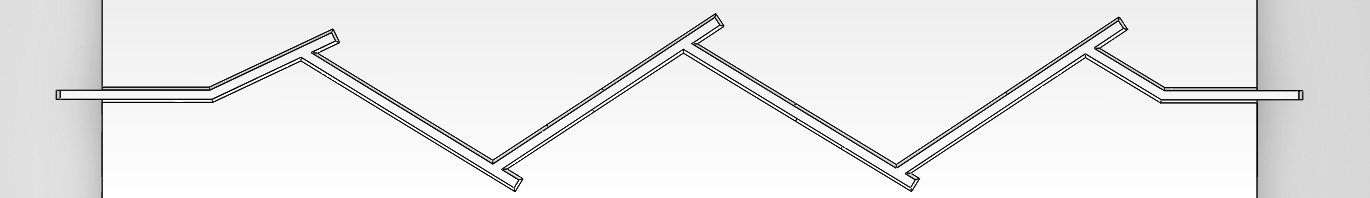
\includegraphics[width=0.19\textwidth]{feature 1.jpeg}}\hfill
  \subfloat[F2]{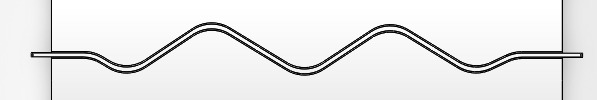
\includegraphics[width=0.19\textwidth]{feature 2.jpeg}}\hfill
  \subfloat[F3]{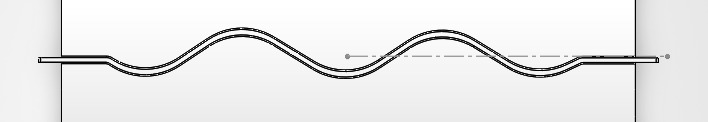
\includegraphics[width=0.19\textwidth]{feature 3.jpeg}}\hfill
  \subfloat[F4 (Perseverance-like)]{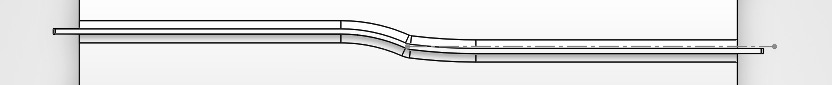
\includegraphics[width=0.19\textwidth]{feature 4.jpeg}}\hfill
  \subfloat[F5]{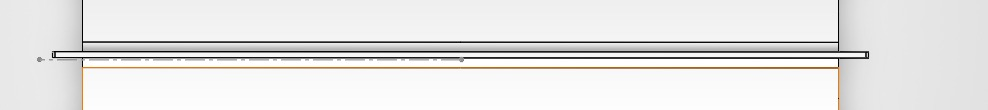
\includegraphics[width=0.19\textwidth]{feature 5.jpeg}}
  \caption{Plan-view grouser profiles of the five features modelled on the curved R250 panel.}
  \label{fig:features}
\end{figure*}

\begin{figure}[!t]
  \centering
  % screenshots cropped to the model viewport (trim = left bottom right top, in bp)
  \subfloat[Flat segment, $a = \SI{2}{mm}$: linearized stress path]{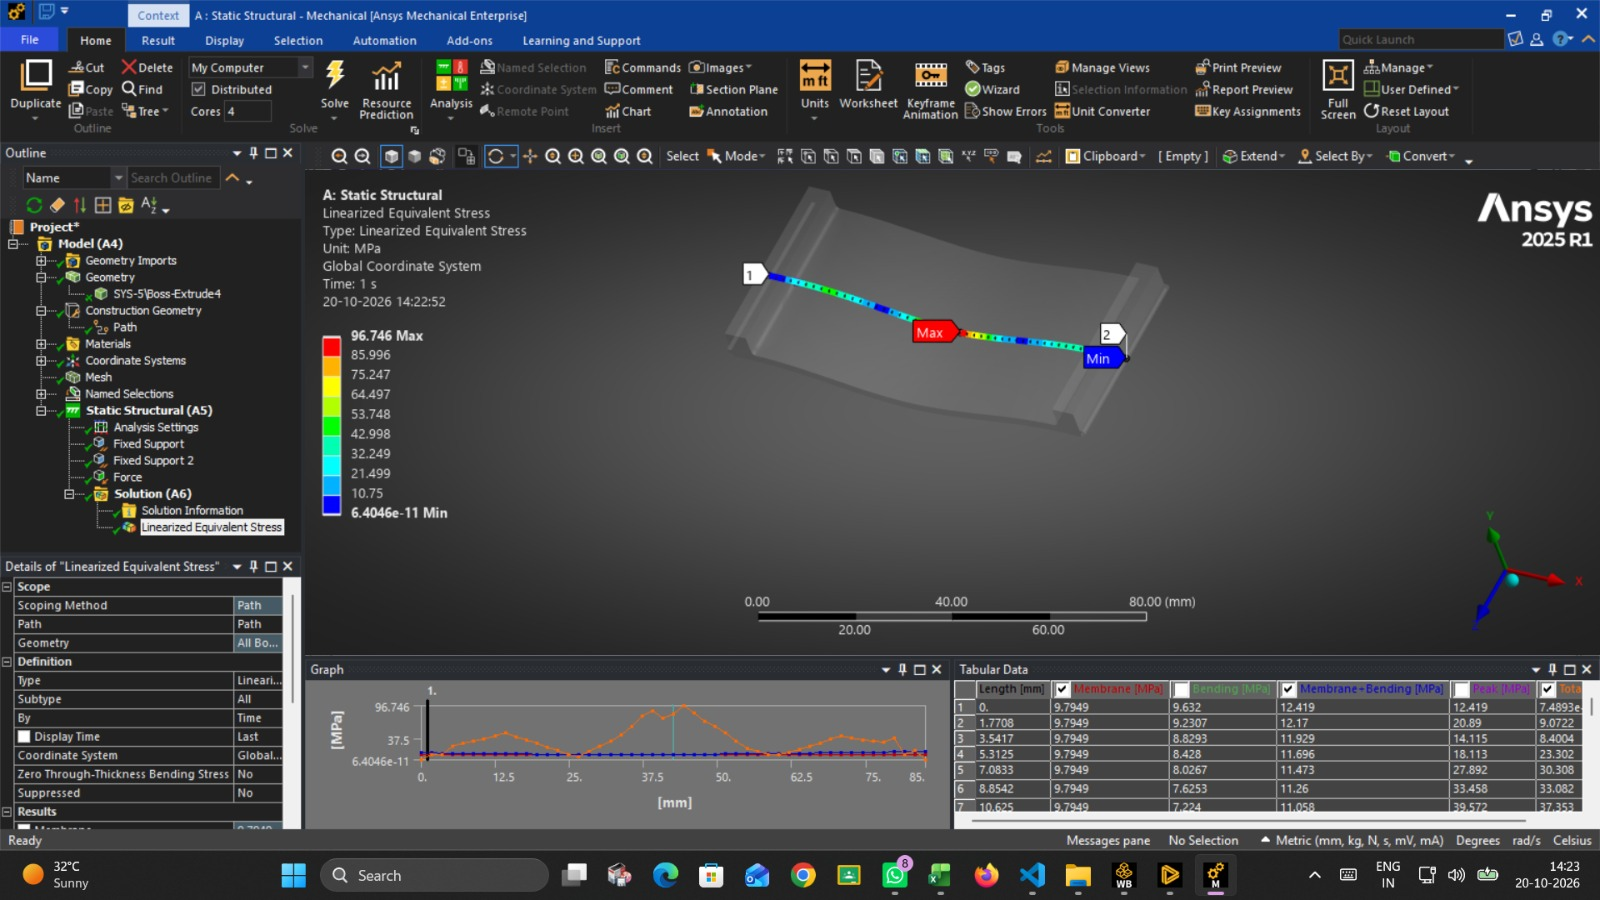
\includegraphics[width=0.48\columnwidth,trim=670 338 290 250,clip]{fea run ex1 tier1.jpeg}}\hfill
  \subfloat[Curved panel (Feature~1): total deformation]{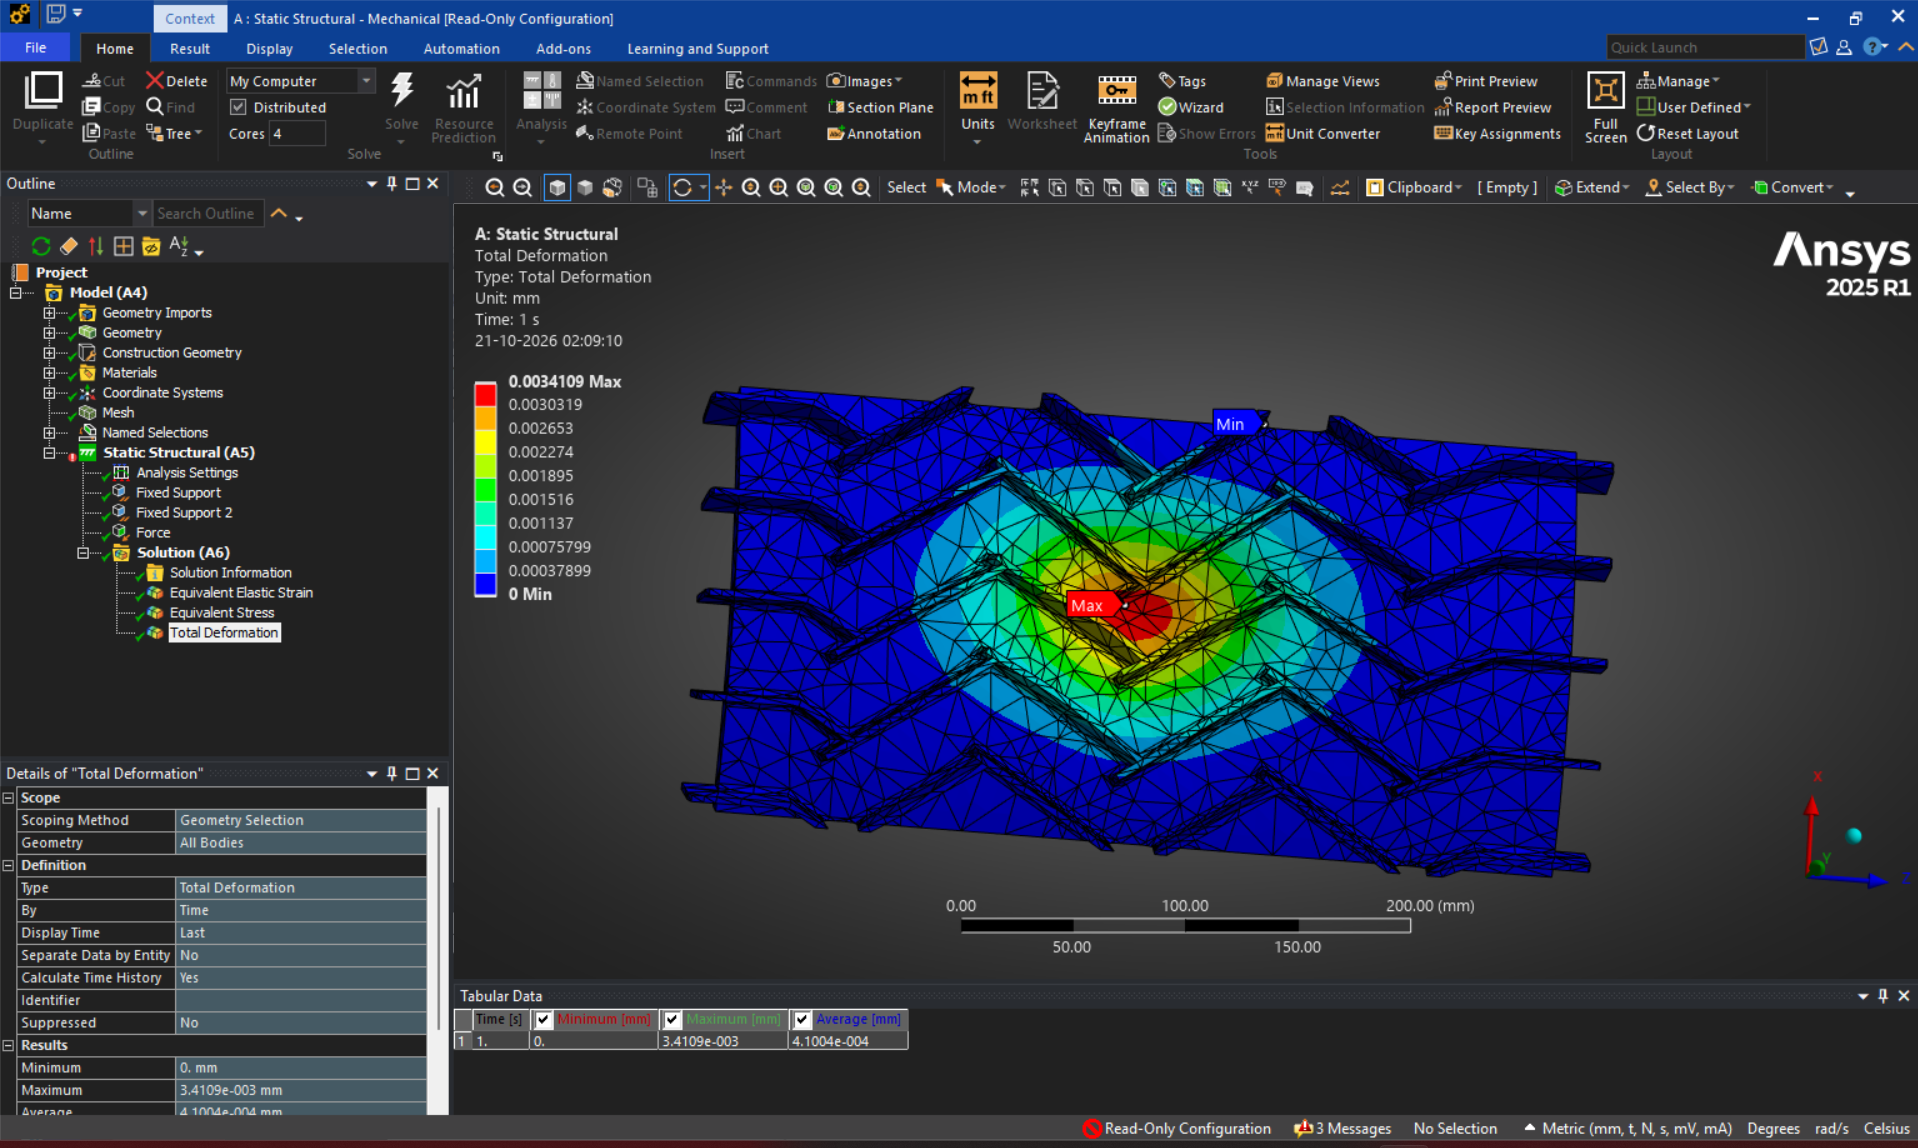
\includegraphics[width=0.48\columnwidth,trim=402 155 176 222,clip]{deformation sim.png}}
  \caption{Sample Ansys Mechanical 2025 R1 runs at \SI{300}{N}, cropped to the model; the full screenshots are in~\cite{rep1,rep2}.}
  \label{fig:ansys}
\end{figure}

% ---------------------------------------------------------------
\section{Methods}

\subsection{Analytical stepped-beam model}
Following the beam and plate formulas tabulated by Roark~\cite{roark}, the pressure $P/\pi a^2$ on the patch, integrated across the width, gives a line load along the span
\begin{equation}
  q(x) = \frac{P}{\pi a^2}\, 2\sqrt{a^2 - (x - x_c)^2}, \qquad |x - x_c| \le a .
\end{equation}
The segment is a beam fixed at both ends, with $I = bD^3/12$ in the grouser blocks and $bt^3/12$ over the skin. The two unknown end reactions follow from zero slope and zero deflection at the far clamp, which handles the stepped section without tables and recovers $|M| = PL'/8$ as $a \to 0$ (see~\cite{rep1}). The surface bending stress $\sigma_\text{nom} = 6M/(bt^2)$ is raised at the junction by Peterson's factor for a shouldered flat bar in bending~\cite{peterson}, $K_t = 1.63$:
\begin{equation}
  \sigma_\text{max} = K_t\, \sigma_\text{nom} .
\end{equation}
The top surface is traction-free and a wide plate in cylindrical bending is restrained laterally ($\sigma_y = \nu\sigma_x$), so the von Mises stress is
\begin{equation}
  \sigma_\text{vm} = |\sigma_x|\sqrt{1 - \nu + \nu^2} .
\end{equation}
The model is in \href{\blob/scripts\%20and\%20outputs/tier_1/path_stress_analytical.m}{\texttt{path\_stress\_analytical.m}}.

\subsection{FEA and mesh convergence}
The flat segment was solved with solid elements, and the stress was extracted as a linearized equivalent stress~\cite{ansys} along a path on the top surface of the skin across the full \SI{85}{mm} span. We use the \emph{Total} column, which is the von Mises stress at each path point, and take the junction peak within \SI{15}{mm} of either end and the centre peak within $\pm\SI{10}{mm}$ of mid-span. Each case was solved on three meshes of nominal element size 10, 1 and \SI{0.1}{mm}, with the geometry, load and path unchanged, so any difference between them comes from the mesh alone. The comparison is in \href{\blob/scripts\%20and\%20outputs/tier_1/fea_vs_analytical.m}{\texttt{fea\_vs\_analytical.m}}.

\subsection{Surrogate model}
Machine-learning surrogates of finite element models have been used to estimate the dynamic response of mechanical systems~\cite{hashemi}. We apply the same idea to skin stress. Each curved-panel case is exported on its own mesh, so every node is mapped to the arc length $u = 250\,\text{atan2}(X, Y)$ and the axial position $Z$, and binned onto a fixed $33 \times 69$ grid of \SI{6}{mm} cells that keep the largest nodal value (Fig.~\ref{fig:pipeline}). The $\log_{10}$ fields are compressed by principal component analysis into 40 shape modes (98.9\% of the variance for stress, 99.4\% for strain), and each mode score is learnt by its own Gaussian process with an ARD squared-exponential kernel in MATLAB \texttt{fitrgp}~\cite{fitrgp}. The nine inputs are the one-hot feature, a thickness flag and $s$, $r$ and $\log R$ scaled to $[0, 1]$. Because the cells and the mode truncation both smooth sharp peaks, one more GP models $\log_{10}$ of the nodal peak directly and gives its 95\% band. The force is not an input: every output is scaled by $F/300$. The model is validated by five-fold cross-validation grouped by stem (one CAD geometry with all five $R$), so every test case is an unseen geometry. Training is in \href{\blob/scripts\%20and\%20outputs/tier_3/train_surrogate.m}{\texttt{train\_surrogate.m}}.

\begin{figure}[!t]
  \centering
  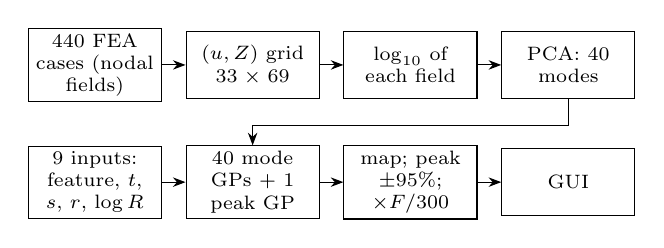
\begin{tikzpicture}[
      box/.style={draw, rectangle, align=center, font=\scriptsize, minimum height=0.85cm, text width=1.55cm, inner sep=2pt},
      >={Stealth[length=1.6mm]}, node distance=0.3cm]
    \node[box] (fea) {440 FEA cases (nodal fields)};
    \node[box, right=of fea] (grid) {$(u,Z)$ grid $33\times69$};
    \node[box, right=of grid] (log) {$\log_{10}$ of each field};
    \node[box, right=of log] (pca) {PCA: 40 modes};
    \node[box, below=0.55cm of fea] (x) {9 inputs: feature, $t$, $s$, $r$, $\log R$};
    \node[box, right=of x] (gps) {40 mode GPs + 1 peak GP};
    \node[box, right=of gps] (out) {map; peak $\pm$95\%; $\times F/300$};
    \node[box, right=of out] (gui) {GUI};
    \draw[->] (fea) -- (grid); \draw[->] (grid) -- (log); \draw[->] (log) -- (pca);
    \draw[->] (pca.south) |- ([yshift=2.5mm]gps.north) -- (gps.north);
    \draw[->] (x) -- (gps); \draw[->] (gps) -- (out); \draw[->] (out) -- (gui);
  \end{tikzpicture}
  \caption{Surrogate pipeline, one copy each for stress and strain (82 GPs in all).}
  \label{fig:pipeline}
\end{figure}

% ---------------------------------------------------------------
\section{Failure Analysis of the Curiosity Skin}

\paragraph*{Mesh convergence}
The \SI{10}{mm} mesh gives results that are an artefact of the mesh: its elements are five times the skin thickness and larger than the patch for $a \le \SI{4}{mm}$, so its peaks are 25--75\% too low at the centre and two to five times too low at the junction, and not even monotonic in $a$ (Fig.~\ref{fig:conv}). From \SI{1}{mm} to \SI{0.1}{mm} the centre peak changes by at most 0.6\% and the junction peak by at most 7.4\%, since a \SI{1}{mm} element is as large as the fillet that causes the concentration. The \SI{0.1}{mm} mesh is therefore used for every conclusion; the full convergence table and the apparent orders of convergence are in~\cite{rep1}.

\begin{figure}[!t]
  \centering
  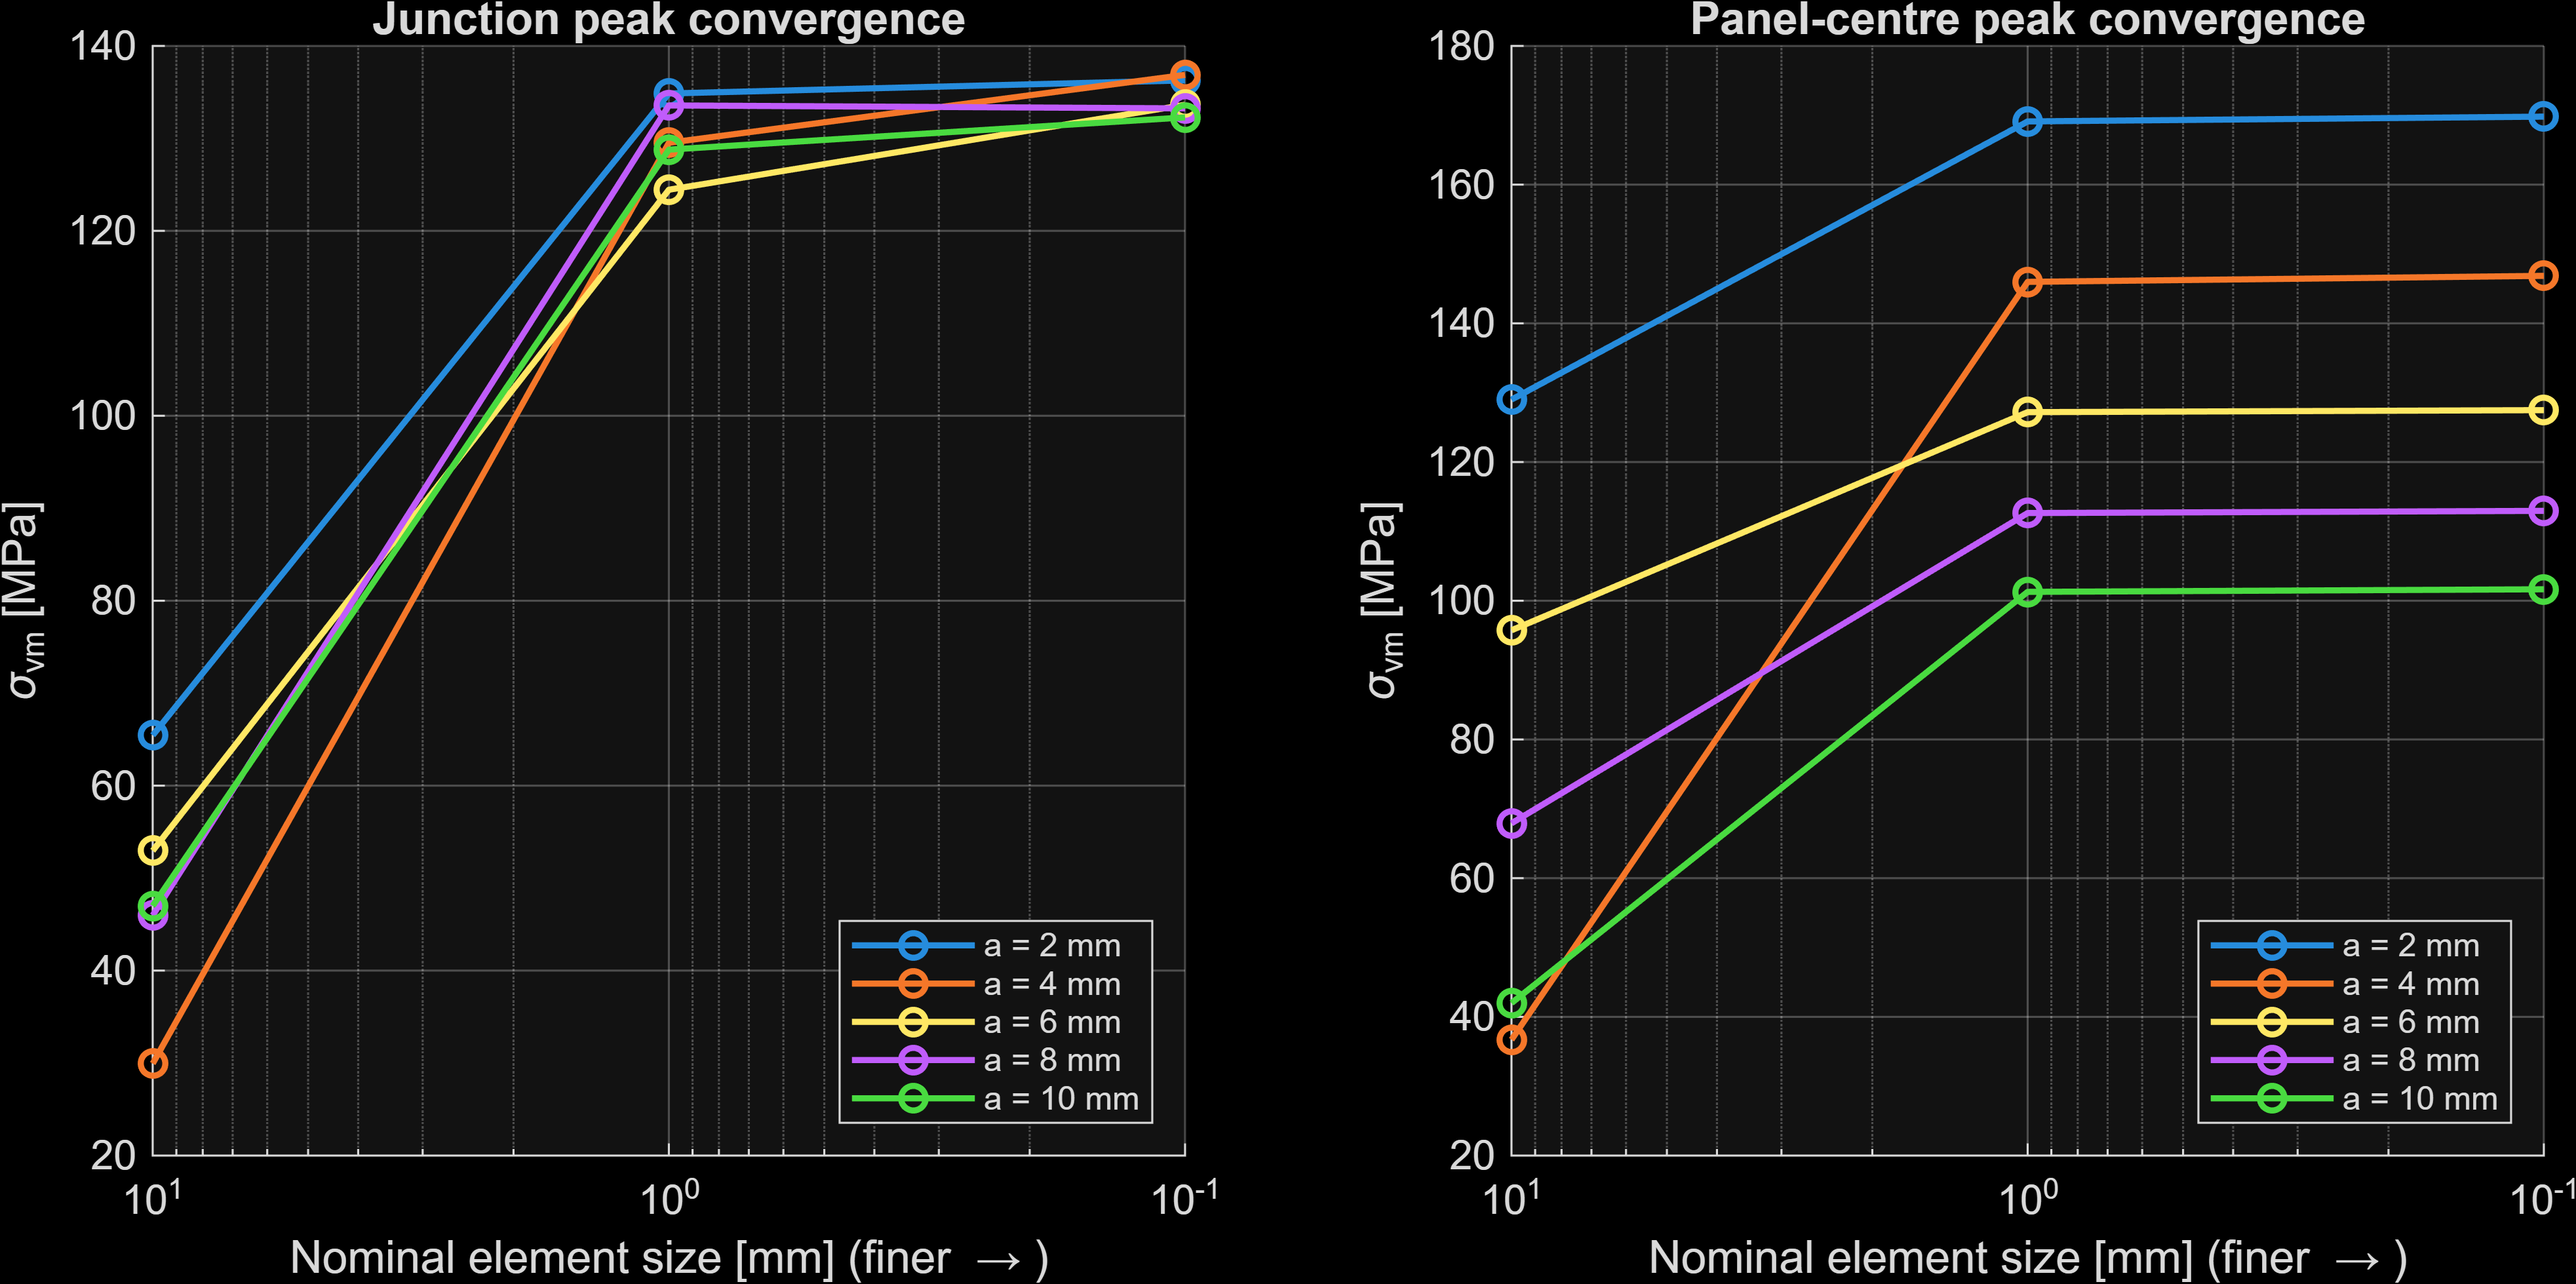
\includegraphics[width=\columnwidth]{mesh_convergence.png}
  \caption{FEA junction (left) and centre (right) peaks against element size, one curve per patch radius, at \SI{400}{N}.}
  \label{fig:conv}
\end{figure}

\begin{table}[!t]
  \centering
  \caption{Converged (\SI{0.1}{mm}) FEA against analytical peaks, MPa at \SI{400}{N}; $C = \sigma_\text{FEA}/\sigma_\text{analytical}$}
  \label{tab:calib}
  \small
  \setlength{\tabcolsep}{4pt}
  \begin{tabular}{rrrrrrr}
    \toprule
    $a$ (mm) & FEA $j$ & An.\ $j$ & $C_j$ & FEA $c$ & An.\ $c$ & $C_c$ \\
    \midrule
    2 & 136.3 & 195.9 & 0.70 & 169.8 & 115.6 & 1.47 \\
    4 & 136.9 & 195.4 & 0.70 & 146.8 & 110.3 & 1.33 \\
    6 & 133.6 & 194.7 & 0.69 & 127.5 & 105.1 & 1.21 \\
    8 & 133.2 & 193.7 & 0.69 & 113.0 & 100.1 & 1.13 \\
    10 & 132.3 & 192.3 & 0.69 & 101.6 & 95.3 & 1.07 \\
    \bottomrule
  \end{tabular}
\end{table}

\paragraph*{Panel centre}
The beam model under-predicts the centre stress at every radius, by 32\% at $a = \SI{2}{mm}$ falling to 6\% at $a = \SI{10}{mm}$ (Table~\ref{tab:calib}). The beam spreads the load over the full \SI{40}{mm} width, while the real plate carries it more locally, and the effect is strongest for the sharpest contact. The beam is thus non-conservative under a sharp rock.

\paragraph*{Junction}
The $K_t$-amplified beam stress is about 1.45 times the FEA value ($C_j \approx 0.7$ for every $a$). The FEA junction peak is 1.12--1.14 times the nominal von Mises stress without $K_t$, so the clamp and width simplifications are not the source of the error; it sits in $K_t$. Peterson's chart is for a symmetric shoulder, which is more severe than this one-sided T-junction, and the path sampling (\SI{1.77}{mm}) may step over the true peak of the \SI{1}{mm} fillet, so the FEA junction values may be a lower bound.

\paragraph*{Implications}
At \SI{400}{N} the junction (132--\SI{137}{MPa}) is above the fatigue limit for every patch size. The centre governs for sharp rocks ($a \le \SI{4}{mm}$: 170 and \SI{147}{MPa}) and falls just below the limit at $a = \SI{10}{mm}$. Cracks would therefore start under the rock only for sharp rocks, and at the junction otherwise, which matches where damage has been reported in service.

% ---------------------------------------------------------------
\section{Curiosity vs Perseverance Design Study}

Table~\ref{tab:design} gives the median FEA peak stress of the curved panel over all grouser angles and fillet radii. Under a sharp rock ($R = \SI{2}{mm}$) the Curiosity-like panel reaches \SI{86}{MPa}, about \SI{115}{MPa} when scaled to \SI{400}{N}, which is above the fatigue limit and agrees with Section~IV. The two Perseverance changes act in sequence. At \SI{2}{mm}, changing the grouser pattern from Feature~1 to Feature~4 alone more than halves the peak (86 to \SI{33}{MPa}), because the ribs share the load. Increasing the skin to \SI{7.5}{mm} then lowers it to \SI{19}{MPa}, about 4.5 times below Curiosity, and below \SI{6}{MPa} for blunter rocks. Every \SI{7.5}{mm} design stays far below the fatigue limit even at \SI{400}{N}. Only stress is assessed; mass is outside this study.

\begin{table}[!t]
  \centering
  \caption{Median FEA peak von Mises stress (MPa) at \SI{300}{N} over all $s$ and $r$. Bold: Curiosity-like and Perseverance-like}
  \label{tab:design}
  \footnotesize
  \setlength{\tabcolsep}{2.4pt}
  \begin{tabular}{l rrrrr rrrrr}
    \toprule
    & \multicolumn{5}{c}{$t = \SI{2}{mm}$, $R$ (mm)} & \multicolumn{5}{c}{$t = \SI{7.5}{mm}$, $R$ (mm)} \\
    \cmidrule(lr){2-6}\cmidrule(lr){7-11}
    & 2 & 4 & 6 & 8 & 10 & 2 & 4 & 6 & 8 & 10 \\
    \midrule
    F1 & \textbf{86.2} & \textbf{54.6} & \textbf{40.4} & \textbf{37.3} & \textbf{29.1} & 17.4 & 4.5 & 3.7 & 3.1 & 2.7 \\
    F2 & 84.1 & 54.9 & 41.0 & 33.5 & 32.0 & 17.0 & 4.8 & 3.7 & 3.2 & 3.2 \\
    F3 & 73.7 & 46.6 & 35.5 & 39.2 & 25.7 & 16.7 & 4.8 & 3.6 & 3.1 & 3.5 \\
    F4 & 33.3 & 26.1 & 28.0 & 25.5 & 25.3 & \textbf{19.2} & \textbf{6.0} & \textbf{4.8} & \textbf{4.4} & \textbf{4.0} \\
    F5 & 20.4 & 21.9 & 18.8 & 19.9 & 18.1 & 13.2 & 5.0 & 3.1 & 2.6 & 2.3 \\
    \bottomrule
  \end{tabular}
\end{table}

% ---------------------------------------------------------------
\section{Surrogate Performance}

Table~\ref{tab:cv} lists the cross-validated metrics; the per-feature breakdown is in~\cite{rep2}. The surrogate predicts the peak stress with a median error of 3.1\%, nine cases in ten are within 11.3\%, and the 95\% band holds the true peak in 93.6\% of cases, close to nominal, so it is a realistic error bar. The whole-map $R^2$ is lower because it also scores the background and the exact location of hot spots. In Fig.~\ref{fig:parity} the points follow the line over more than a decade, and the largest scatter is in the 3--\SI{8}{MPa} cluster of stiff \SI{7.5}{mm} panels, where absolute errors are small.

\begin{table}[!t]
  \centering
  \caption{Five-fold stem-grouped cross-validation, all 440 cases}
  \label{tab:cv}
  \footnotesize
  \setlength{\tabcolsep}{3pt}
  \begin{tabular}{lcccccccc}
    \toprule
    & \multicolumn{2}{c}{Field $R^2$} & \multicolumn{2}{c}{Peak $R^2$} & \multicolumn{2}{c}{Peak err.\ (\%)} & Cov. \\
    \cmidrule(lr){2-3}\cmidrule(lr){4-5}\cmidrule(lr){6-7}
    Field & lin & log & lin & log & med. & P90 & (\%) \\
    \midrule
    Stress & 0.956 & 0.979 & 0.993 & 0.996 & 3.1 & 11.3 & 93.6 \\
    Strain & 0.970 & 0.984 & 0.994 & 0.996 & 3.1 & 10.9 & 93.4 \\
    \bottomrule
  \end{tabular}
\end{table}

\begin{figure}[!t]
  \centering
  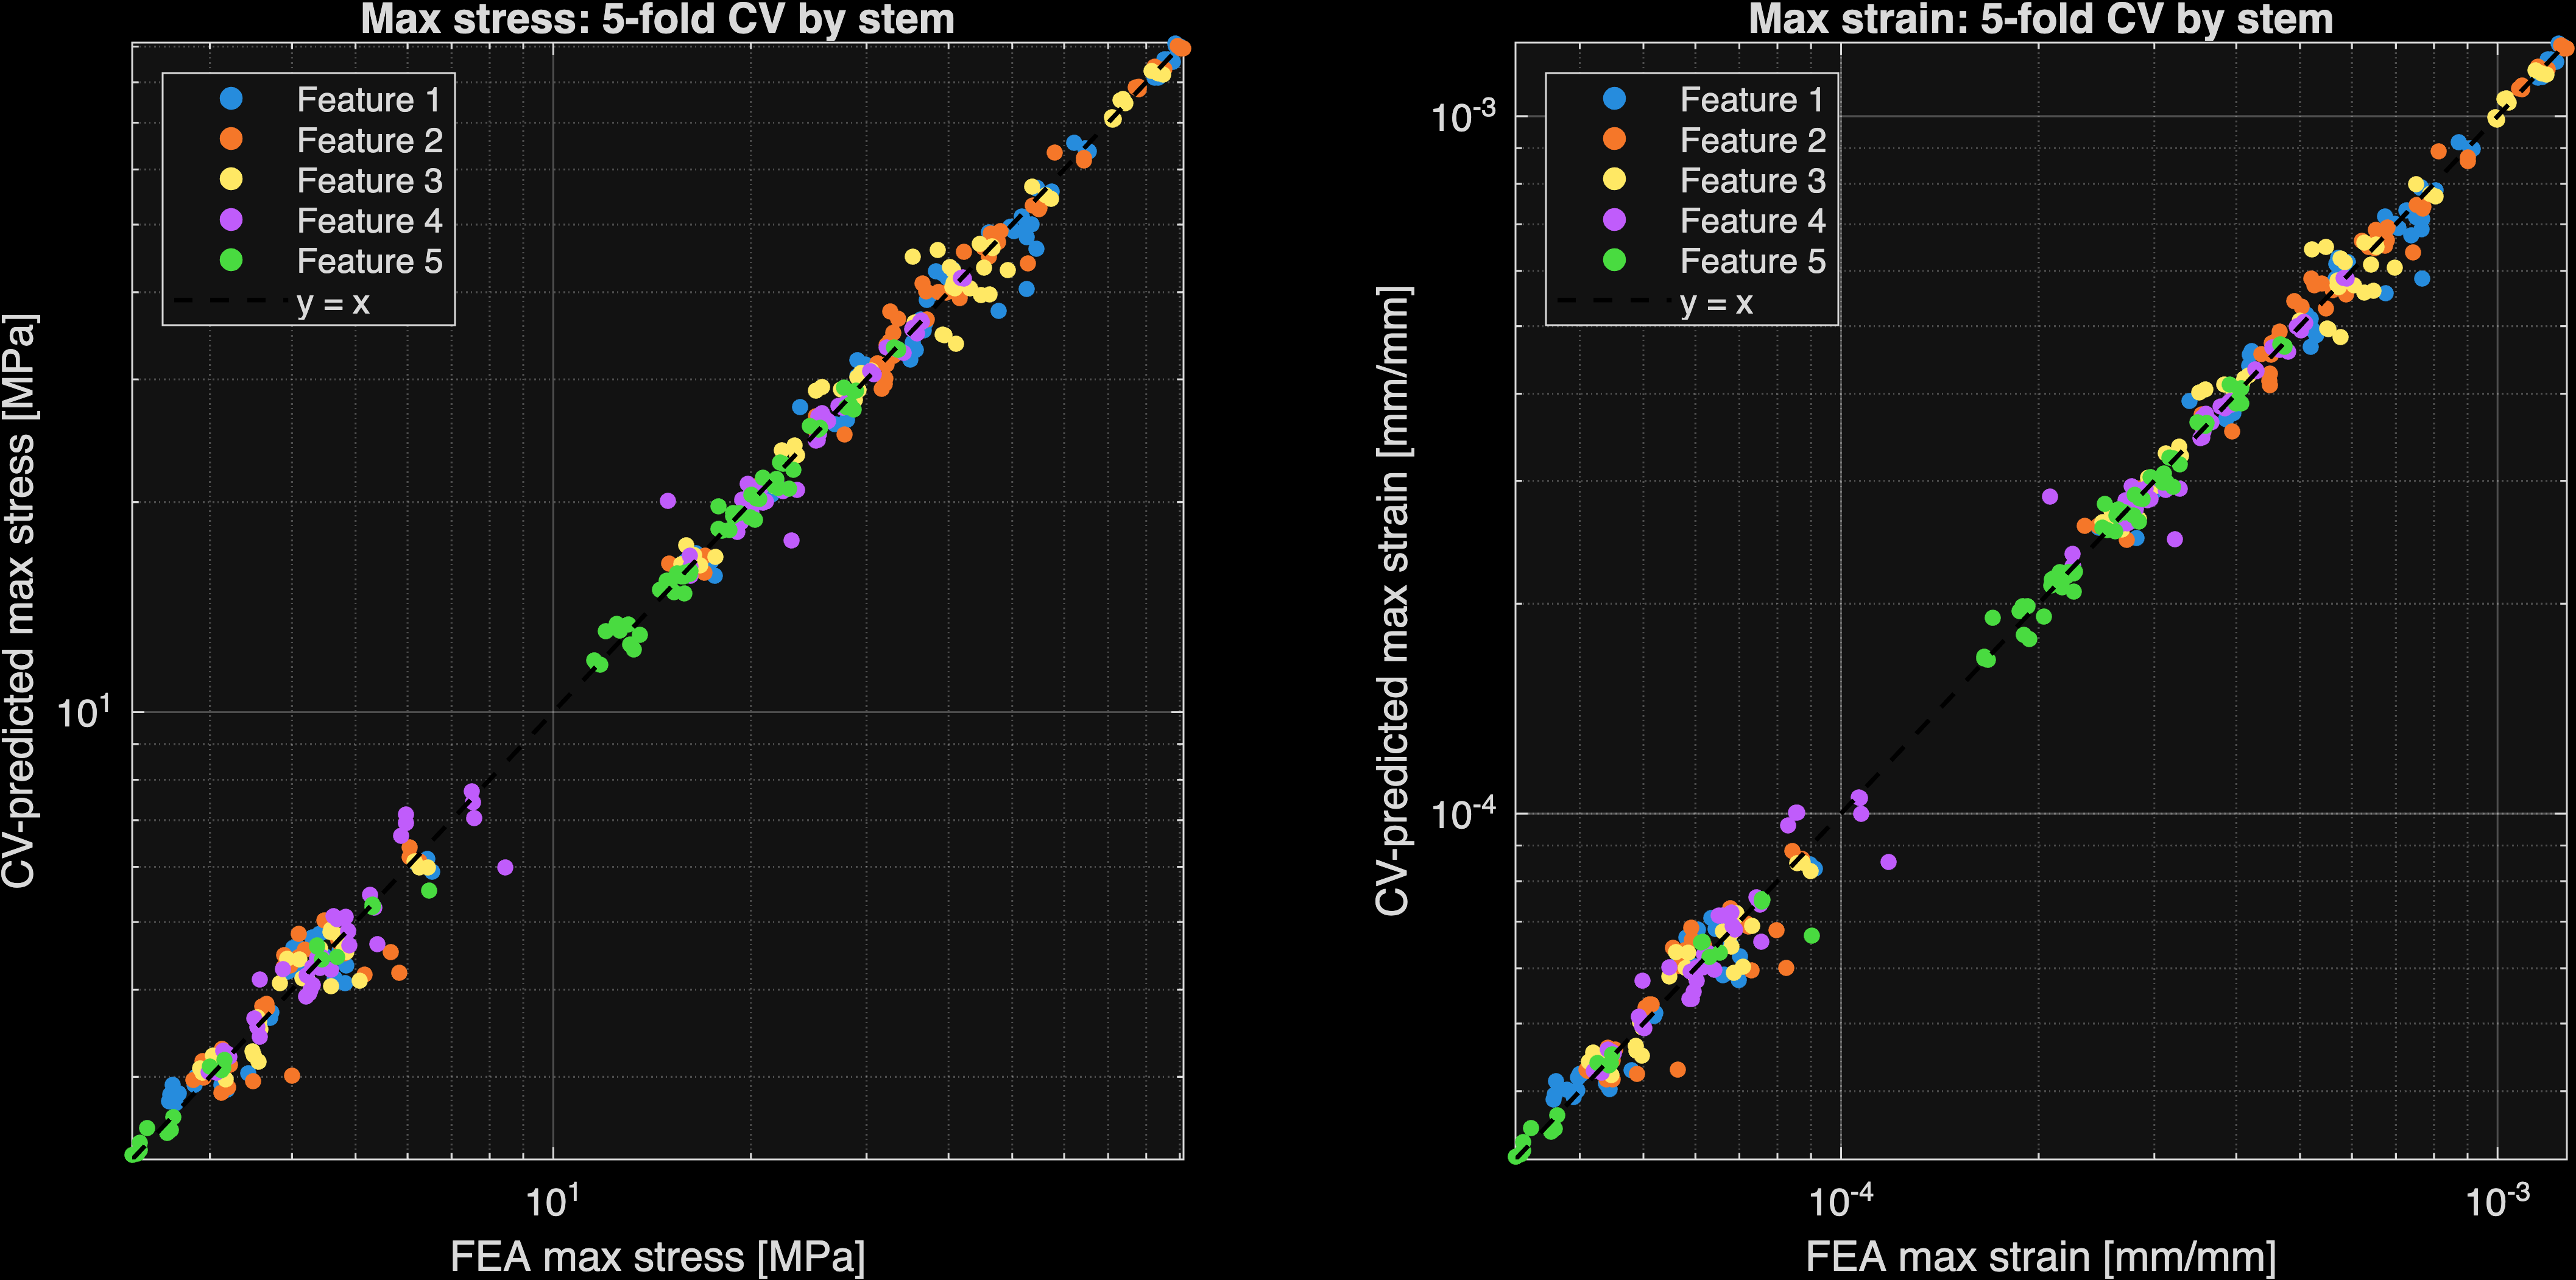
\includegraphics[width=\columnwidth]{cv_parity_max.png}
  \caption{Cross-validated peak stress (left) and strain (right) against FEA, coloured by feature, on log axes.}
  \label{fig:parity}
\end{figure}

The GUI, \href{\blob/scripts\%20and\%20outputs/tier_3/tier3_gui.m}{\texttt{tier3\_gui.m}} (Fig.~\ref{fig:gui}), takes the feature, $t$, $s$, $r$, $R$ and $F$, flags each input as simulated, interpolated or out of range, and shows the predicted maps and peaks with their 95\% band next to the nearest solved FEA case. In the example shown the surrogate predicts \SI{37.9}{MPa} [33.2, 43.2], and the nearest FEA case gives \SI{35.5}{MPa}. The predicted maps are \SI{6}{mm} cell maxima, so the local fillet value should be read from the peak model. Feature and thickness are categories, so a new grouser profile or an intermediate thickness cannot be predicted, and between $s = 10$ and \SI{12}{\degree} the model blends a five- and a three-grouser layout.

\begin{figure}[!t]
  \centering
  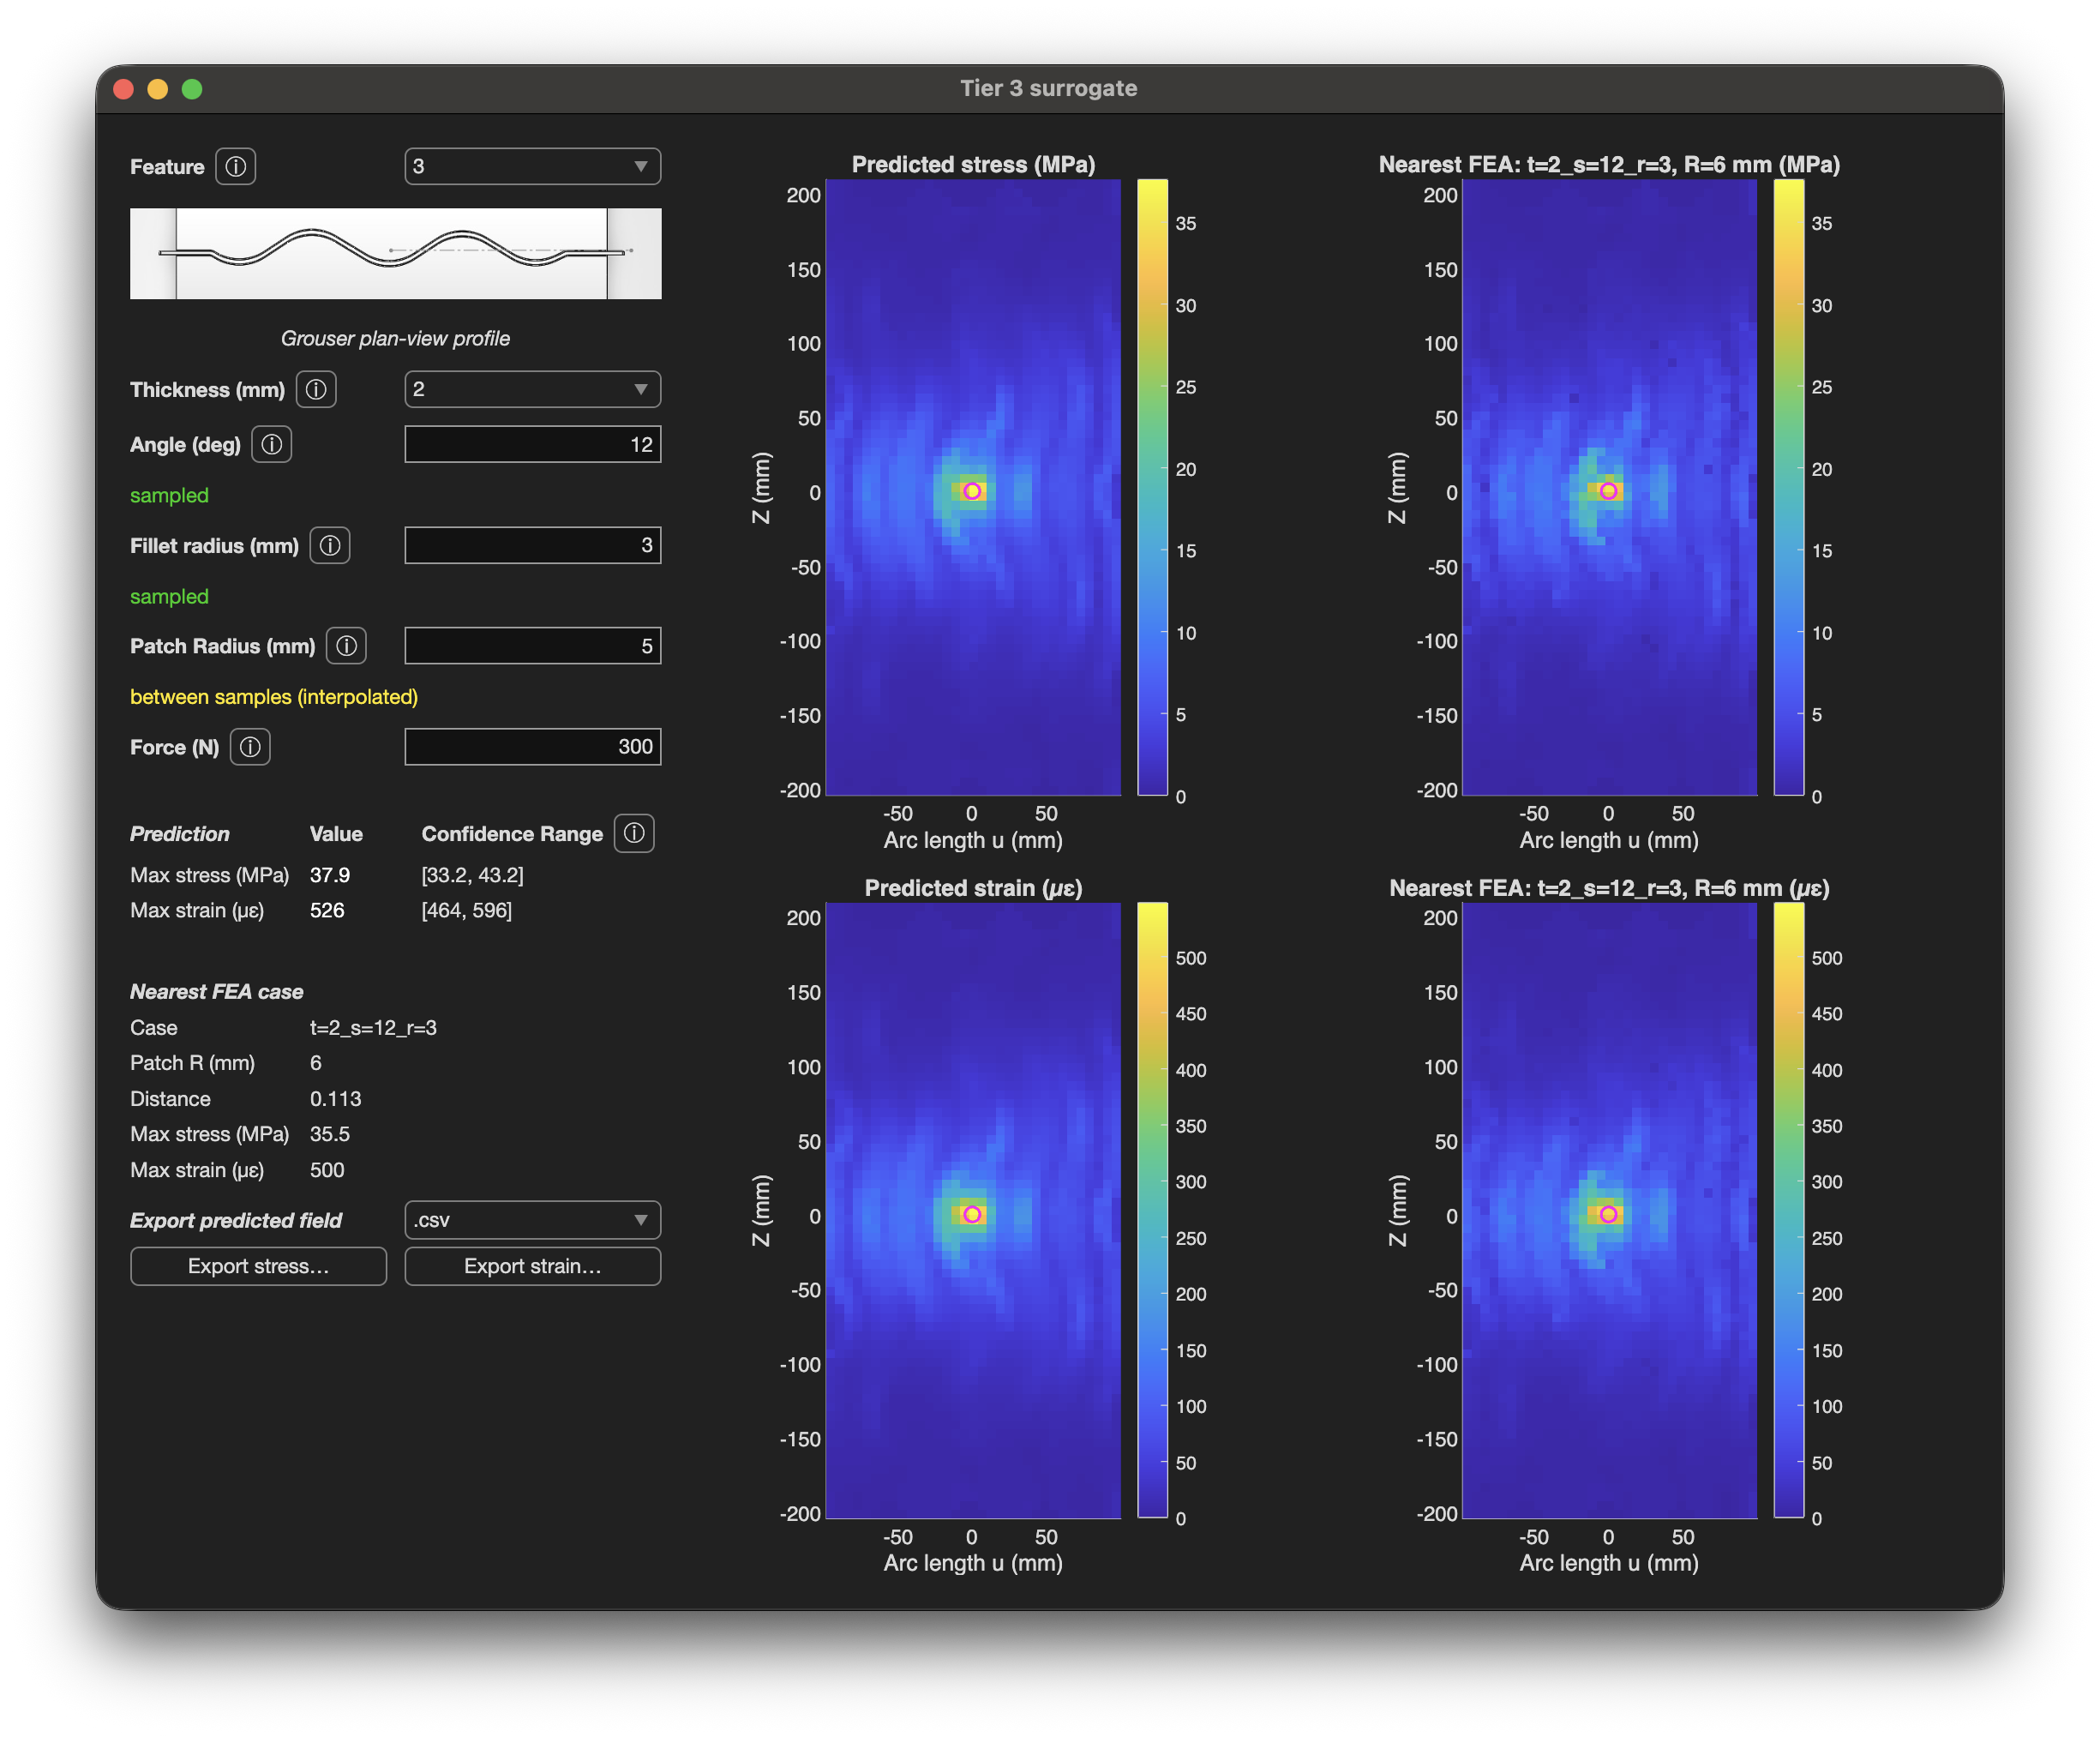
\includegraphics[width=\columnwidth]{Surrogate GUI.png}
  \caption{Surrogate GUI: Feature~3, $t = \SI{2}{mm}$, $s = \SI{12}{\degree}$, $r = \SI{3}{mm}$, $R = \SI{5}{mm}$, \SI{300}{N}. The elements are described in~\cite{rep2}.}
  \label{fig:gui}
\end{figure}

% ---------------------------------------------------------------
\section{Conclusions}

A rock pressing on the Curiosity skin between two grousers bends it like a clamped strip, and at \SI{400}{N} the stress at the skin--grouser junction is above the fatigue limit for every rock size, while the stress under the rock is above it for sharp rocks. This matches where cracks have been reported. A hand calculation captures the pattern but under-estimates the stress under sharp rocks and over-estimates it at the junction, and the FEA is only trustworthy once the mesh is fine enough to resolve the \SI{2}{mm} skin and its fillet. Both Perseverance changes reduce the stress: the ribbed grouser pattern more than halves the sharp-rock peak on a \SI{2}{mm} skin (86 to \SI{33}{MPa}), and the \SI{7.5}{mm} skin brings it down to \SI{19}{MPa}, closing the fatigue problem. The surrogate reproduces the FEA closely enough for screening, and its natural next use is optimisation, i.e.\ finding the thinnest skin or the grouser angle and fillet that keep the peak below the limit for a given rock and load.

\section*{AI Disclosure}
Generative AI tools (Anthropic's Claude Code) were used to assist with scripting, document preparation and editing of this paper. The authors are responsible for all results and conclusions. The scripts, data and results behind every figure and number, along with details of AI use, are available in the project repository~\cite{repo}.

\clearpage
\onecolumn   % references span the full page width on the last page
\begin{thebibliography}{9}\scriptsize   % smaller reference font
  \bibitem{repo} P.~K.~Sahoo, R.~Bagul, S.~Panda and Shaswath~S, ``Curiosity--Perseverance wheel FEA,'' GitHub repository. \url{\repo}
  \bibitem{rep1} P.~K.~Sahoo, R.~Bagul, S.~Panda and Shaswath~S, ``Curiosity rover wheel failure analysis,'' detailed report. \href{\blob/latex/Failure\%20analysis/report.pdf}{\texttt{latex/Failure analysis/report.pdf}}
  \bibitem{rep2} P.~K.~Sahoo, R.~Bagul, S.~Panda and Shaswath~S, ``Curiosity to Perseverance rover wheels: surrogate modelling of skin stress and strain,'' detailed report. \href{\blob/latex/Surrogate\%20Model/report.pdf}{\texttt{latex/Surrogate Model/report.pdf}}
  \bibitem{nasa} NASA Jet Propulsion Laboratory, Mars Science Laboratory (Curiosity) and Mars 2020 (Perseverance) mission reports and status updates on wheel wear. \url{https://mars.nasa.gov/}
  \bibitem{roark} W.~C.~Young and R.~G.~Budynas, \emph{Roark's Formulas for Stress and Strain}, 7th~ed. New York: McGraw-Hill, 2002.
  \bibitem{peterson} W.~D.~Pilkey and D.~F.~Pilkey, \emph{Peterson's Stress Concentration Factors}, 3rd~ed. Hoboken, NJ: Wiley, 2008.
  \bibitem{ansys} Ansys Inc., \emph{Ansys Mechanical User's Guide, Release 2025 R1}: Linearized Stress.
  \bibitem{fitrgp} The MathWorks, \emph{Statistics and Machine Learning Toolbox User's Guide}: \texttt{fitrgp}, Gaussian process regression.
  \bibitem{hashemi} A.~Hashemi, J.~Jang and J.~Beheshti, ``A machine learning-based surrogate finite element model for estimating dynamic response of mechanical systems,'' \emph{IEEE Access}, 2023. \url{https://doi.org/10.1109/ACCESS.2023.3282453}
\end{thebibliography}

\end{document}
